\documentclass[]{report}
\usepackage{amsmath}
\usepackage{amssymb}
\usepackage[english]{babel}
\usepackage[utf8]{inputenc}
\usepackage[T1]{fontenc}
\usepackage{euler}

\usepackage[inner=0cm,outer=0cm,top=0.1cm,bottom=0cm,paperwidth=6.5cm,paperheight=6.5cm]{geometry}

\usepackage{tikz,pgfplots}
\usetikzlibrary{positioning}
\usetikzlibrary{decorations.pathmorphing}

\begin{document}
\centering
	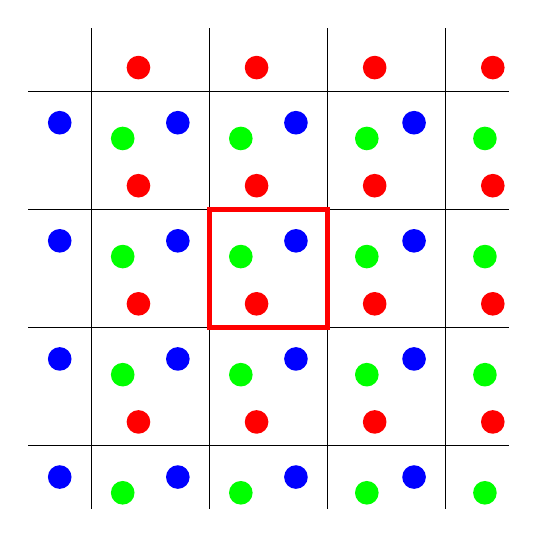
\begin{tikzpicture}
		\draw[step=1.5cm,thin] (-0.8,-0.8) grid (5.3,5.3);
		\draw[draw=red,ultra thick] (1.5,1.5) rectangle (3,3);
		\foreach \x in 	{0.6,2.1,3.6,5.1}
			\foreach \y in {0.3,1.8,3.3,4.8}
				\fill[fill=red] (\x,\y) circle (0.15);
		\foreach \x in 	{-0.4,1.1,2.6,4.1}
			\foreach \y in {-0.4,1.1,2.6,4.1}
				\fill[fill=blue] (\x,\y) circle (0.15);
		\foreach \x in 	{0.4,1.9,3.5,5}
			\foreach \y in {-0.6,0.9,2.4,3.9}
				\fill[fill=green] (\x,\y) circle (0.15);
	\end{tikzpicture}
\end{document}
	